\documentclass[PMI,VKR]{HSEUniversity}
% Возможные опции: KR или VKR; PI или BI

\title{Dynamic Topic Modeling for Voice Dialogues}
\author{Miakov Timofey Ilich}
\supervisor{Professor NRU HSE - Nizhniy Novgorodw}{L.V. Savchenko }
\Year{2024}
\Abstract{

}

\bibliography{library.bib}

\begin{document}

\maketitle

\chapter{Introduction}

\section{Motivation}

\section{Research Objectives}
The objectives of the thesis work are:
\begin{itemize}
    \item A review of existing approaches to dynamic text and dialogue topic modelling
    \item The definition of the main stages for DTM for audio dialogues
    \item The identification of suitable training data sets and their collection
    \item An exploration of the possibilities of using large language models for some stages and the selection of models suitable for training in limited resources
    \item The development of the architecture of all stages and their interconnections
    \item The identification of key indicators to assess the quality of each stage is also required
    \item Visual analysis of the pipeline operation on pre-selected audio data
\end{itemize}


\chapter{Theoretical explanation}

The pipeline of dynamic thematic modelling of audio dialogues, which will be considered in this paper, is divided into several main stages. 
These include audio-to-text, dialogue segmentation, topic extraction, and topic evolution. 
The approaches and algorithms used in these stages will be described in detail from a theoretical point of view.


\section{Automatic Speech Recognition Stage}



\section{Dialogue Segmentation Stage}

The dialogue segmentation stage represents the initial stage for textual type of data. 
At this stage, a set of strings is input, with each line representing an utterance from one dialogue participant. 
The result is a set of utterance indices that indicate the beginning of a thematically related group. 

In accordance with the majority of previous studies, we have utilise the best open-source solution based on the presented in papers metrics. 
Let us now examine the algorithm in greater detail. 

The input of stage is a set of utterances $\{u1, u2, ..., uk\}$, splited into pairs of consecutive utterance. 
All utterances text encode by encoder model.

\subsection{BERT for embeddings extraction}

The BERT model is a Transformer encoder that was first introduced in the article BERT: Pre-training of Deep Bidirectional Transformers for Language Understanding\cite{bert:2018}.  
This article presents a new approach to the learning process and how BERT is used for downstream tasks.

\begin{figure}[h]
    \centering
    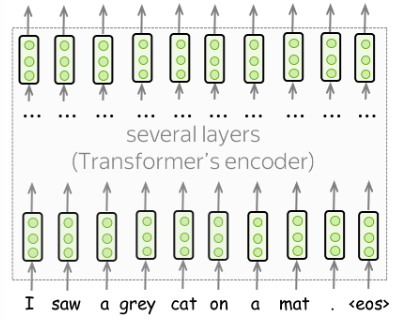
\includegraphics[scale=0.8]{img/bert.png}
    \caption{BERT architecture}
\end{figure}


\begin{figure}[h]
    \centering
    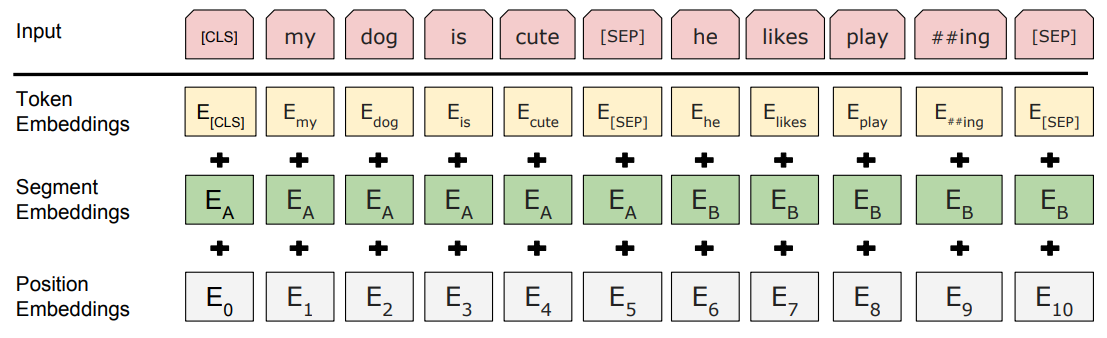
\includegraphics[scale=0.6]{img/bert_input.png}
    \caption{}
\end{figure}

The input data for training comprises pairs of sentences separated by a special token separator [SEP] (Figure 2.15). 
In order to facilitate the model's ability to distinguish between these sentences, it employs segment embeddings in addition to token and position embeddings. 
BERT also has two learning objectives for which some special tokens ([MASK], [CLS]) are used. 

The first objective of the training process is the masked language modelling (MLM). 
During the learning phase of MLM, the following occurs:

\begin{itemize}
    \item A number of tokens are selected with a probability of 15\% for each token.
    \item The selected tokens are replaced by [MASK] with a probability of 80\%, a random token with a probability of 15\% and remain unchanged with a probability of 10\%.
    \item The model must predict the original token.
\end{itemize}

The figure below illustrates an example of a training step for a single sentence.

The Next Sentence Prediction (NSP) task is a binary classification task. 
In order to understand relationship between two sentences, BERT training process also uses next sentence prediction.
During training the model gets as input pairs of sentences and it learns to predict if the second sentence is the next sentence in the original text as well. 
The training dataset presented in the original paper states that when trained, 50\% of the examples contain related sentences extracted from the training texts, while the remaining 50\% contain a random pair of sentences.

In terms of our approach to topic segmentation, authors utilise Next Sentence Prediction (NSP) BERT as the encoder, due to the similarity of these two tasks. 
Both tasks take a pair of sentences/utterances as input, with the objective of predicting the appropriate next sentence, which should be topically related. 

In more detail, the positive instances $(s_{i}, s_{t+i})$ and negative instances $(s_{i}, s_{t-i})$ are fed into the model in the form of the following sequence: 
\begin{center}
    $[CLS] s_{i} [SEP] s_{t+/-i} [SEP]$,
\end{center}
where the symbols $[CLS]$ and $[SEP]$ represent special tokens in BERT. 

Here, the contextualised representation of $[CLS]$ is employed as the topic-aware embedding to predict the degree of matching between the two input utterances in terms of topic. 
The topical coherence score is estimated by passing the $[CLS]$ representation through another MLP.


\subsection{Depth Scores calculation}

Subsequently, an utterance-pair coherence scoring model is applied to $k - 1$ consecutive pairs, resulting in a sequence of coherence scores $\{c1, c2, ..., ck-1\}$. 
The value of $c_i \in [0, 1]$ indicates the topical relatedness of the two utterances in the $i_th$ pair. 
The algorithm utilises coherence scores as a foundation idea, yet enhances them through the sequence of "depth scores". $\{dp1, dp2, ..., dpk-1\}$ is calculated to measure the sharpness of a valley. 
This is achieved by examining the highest coherence scores $h_l(i)$ and $h_r(i)$ on either side of interval $i$.

The depth score for interval $i$, $dp_i$, is calculated as follows: 
\begin{center}
    $D_{pi} = \frac{ h_{l}(i) + h_{r}(i) - 2 \cdot c_{i}}{2}$. 
\end{center}

A higher depth score indicates a lower topical relatedness between the pair of utterances. 
The threshold $\tau$, which is used to identify segment boundaries, is computed from the mean $\mu$ and standard deviation $\sigma$ of depth scores: $\tau = \mu - \frac{\sigma}{2}$. 
A pair of utterances with a depth score exceeding $\tau$ will be selected to have a segment boundary between them. 


\section{Topic Extraction Stage}


\subsection{Methods overview}


\subsection{Large Language Models}


\subsection{LLM for topic extraction}


\section{Topic Evolution over time}



\section{Attention mechanism}

Механизм внимания является частью нейронной сети. На каждом этапе декодирования он решает, какие части входных данных важнее всего. При этом кодировщику не нужно сжимать весь исходный код в один вектор - он создает представления для всех токенов источника.

\begin{figure}[h]
    \centering
    \includegraphics[scale=0.3]{img/transformer/attention_mech1.png}
    \caption{Схема работы механизма внимания}
\end{figure}

\newpage
Алгоритм работы механизма внимания в encoder-decoder модели приведен ниже.

\begin{itemize}
    \item На каждом этапе декодирования механизм внимания получает на вход: состояние декодера $h_t$ и все состояния кодировщика $s_1, s_2, \dots, s_m$
    \item Вычисляет коэффициенты внимания (attention scores) для каждого состояния кодеровщика $s_k$ механизм внимания вычисляет свою "релевантность" для этого состояния декодера $h_t$. \\
          Для вычисления можно применить любую функцию, однако, есть несколько популярных и простых вариантов, которые работают довольно хорошо.
          \begin{itemize}
              \item $scores(h_t, s_k) = h_t^T \cdot s_k $
              \item $scores(h_t, s_k) = h_t^T \cdot W \cdot s_k $, где $W$ - матрица (обучаемый параметр)
              \item $scores(h_t, s_k) = w_2^T \cdot \tanh(W \cdot [h_t^T, s_k]) $, где $W, w_2$ - матрицы (обучаемые параметры), а $[h_t^T, s_k]$ означает конкатенацию векторов
          \end{itemize}

    \item Вычисляет веса внимания (attention weights): распределение вероятностей - softmax, применяемое к показателям внимания;
    \item Вычисляет вывод внимания : взвешенная сумма состояний декодера с весами внимания.
\end{itemize}

\begin{figure}[h]
    \centering
    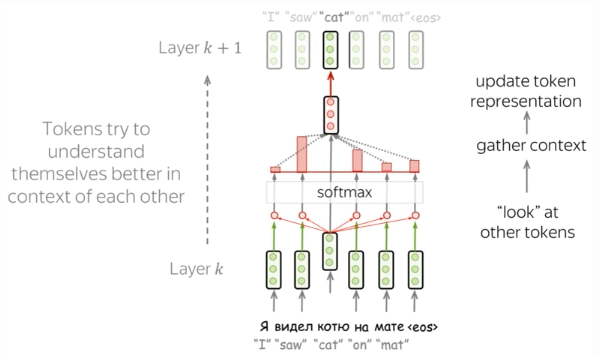
\includegraphics[scale=1]{img/transformer/self-attention.png}
    \caption{Схема работы self-attention механизма}
\end{figure}

\subsection{Self-attention}

Self-attention - является одним из ключевых компонентов модели, в которой токены взаимодействуют друг с другом. На каждом шаге в энкодере токены обмениваются информацией между собой, собирает контекст и обновляет предыдущее представление себя (рис 2.3). Такой подход полностью исключает последовательную обработку, как в RNN, что ускоряет работу нейронной сети и дает возможность обрабатывать каждое слово параллельно.

\newpage
\subsection{}

Каждый входной токен в self-attention получает три представления, соответствующие ролям, которые он может играть:
\begin{itemize}
    \item query - запрашивает информацию;
    \item key - показывает, какая информация есть у него;
    \item value - дает запрашиваемую информацию;
\end{itemize}

От слова, которое мы сейчас подаем на вход (центральное), требуется query вектор, этим вектором мы запрашиваем у других информацию о текущем слове в данном контексте. От каждого другого слова нам будет нужен вектор key, который показывает, какую информацию данное слово может сказать о смысле центрального слова, а также вектор value, из которого мы и получим нужную нам информацию.

Получив информацию от каждого вектора, мы подаем это на вход softmax функции и получаем итоговый эмбеддинг центрального слова.
На рисунке нижен представлен полный алгоритм взаимодействия Q, K, V в self-attention механизме.

\newpage
\begin{figure}[h]
    \centering
    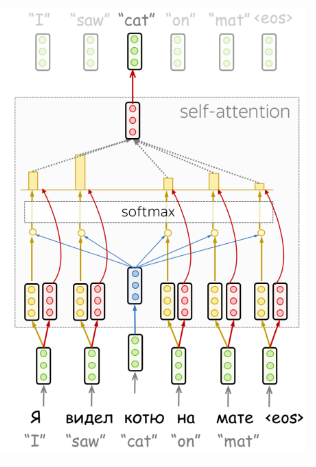
\includegraphics[scale=1]{img/transformer/query-key-value.png}
    \caption{Query, Key, Value в self-attention механизма}
\end{figure}

Формула для вычисления выходных данных внимания следующая:

\begin{center}
    $Attention(q, k, v) = softmax(\frac{q \cdot k^T}{\sqrt{d_k}}) \cdot v $
\end{center}

\subsection{Masked self-attention}

Для энкодера и декодера используются разные способы получения токенов, если энкодер получает все токены сразу и каждый токен может смотреть на любой другой токен во входном предложении, в декодере, мы генерируем по одному токену за раз: во время генерации мы не знаем, какие токены мы будем генерировать в дальше.
Чтобы запретить декодеру заглядывать вперед, модель использует masked-self attention, который видит токены, только стоящие до него во входной последовательности.

Работа masked self-attention отличается во время обучения и инференса модели. Во время второго декодер не заглядывает вперед - так как, мы не знаем, что будет дальше. Но при обучении используются уже известные нам данные. Поэтому при обучении на вход декодеру подется все целевое предложение целиком - без масок.

На рисунке нижне приведен алгоритм работы masked self-attention механизма.

\begin{figure}[h]
    \centering
    \includegraphics[scale=0.9]{img/transformer/masked self-attention.png}
    \caption{Схема работы masked Self-attention механизма}
\end{figure}

\begin{figure}[h]
    \centering
    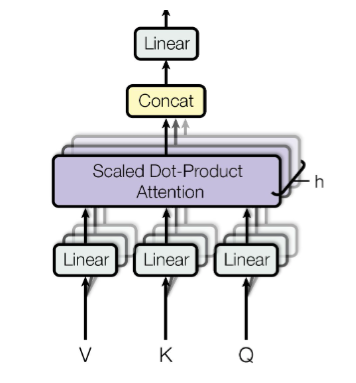
\includegraphics[scale=1]{img/transformer/multi-head.png}
    \caption{Схема Multi-head attention}
\end{figure}

\subsection{Multi-Head Attention}

Обычно понимание роли слова в предложении требует понимания того, как оно связано с разными частями предложения. Это важно не только при обработке исходного предложения, но и при генерации целевого.
Поэтому мы должны позволить модели сосредоточиться на разных вещах: для этого сделали multi-head attention. Вместо одного attention механизма multi-head attention имеет несколько «голов», которые работают независимо.

\begin{center}
    $MultiHead(Q, K, V) = Concat(head_{1}, head_{2}, \dots, head_{n})$ \\
    $head_{i} = Attention(QW^{i}_{Q}, KW^{i}_{K}, VW^{i}_{V})$
\end{center}

Формально это реализовано в виде нескольких механизмов внимания, результаты которых объединяются. (рис 2.6)

\newpage
\section{Трансформер: Архитектура модель}

Трансформер - это модель, основанная только на механизме винмания и оказавшая огромное влияние на NLP в частности и машинном обучении в целом. Впервые представленная в статье Attention is All You Need\cite{allyouneed:2017} в 2017 году.
Модель сразу показала лучшие результаты в задаче перевода, в сравнении с encoder-decoder модели.

\begin{figure}[h]
    \centering
    \includegraphics[scale=0.2]{img/transformer/transformer.png}
    \caption{Схема архитектуры Траснформер}
\end{figure}

Трансформер состоит из частей, которое ранне описывались. Encoder состоит из multi-head self-attention механизмов и генерирует представление слов, а decoder из masked self-attention механизма, который уже генерирует новую последовательность. Это происходит в несколько слоев, обычно 6.

Теперь рассмотрими другие составляющие архитекутры:\\


\subsection{Feed forward and Add $\&$ Norm}

Кроме блоков внимания, в Трансформере также присутствуют feed forward слои, которые состоят из линейного слоя и фукнции активации ReLU.

\begin{figure}[h]
    \centering
    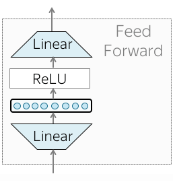
\includegraphics[scale=1]{img/transformer/feed_forward.png}
    \caption{Feed-forward слой}
\end{figure}

Вторым важным слоем является LayerNorm, которой независимо нормализует векторное представление каждой последовательности в батче. В Трансформере нормализуются векторное представление каждого токена. Кроме того, LayerNorm имеет обучаемые параметры, $scale$ и $bias$, которые используются после нормализации для масштабирования выходных данных слоя.

\begin{figure}[h]
    \centering
    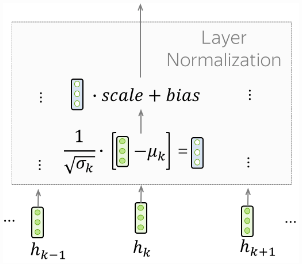
\includegraphics[scale=1]{img/transformer/layer_norm.png}
    \caption{LayerNorm слой}
\end{figure}

На рис 2.8 стоит обратить внимание на то, что $\mu_{k}$ и $\sigma_{k}$ оцениваются для каждой последовательности, в отличии от $scale$ и $bias$, которые являются параметрами слоя.


\subsection{Positional encoding}

Поскольку Transformer не знает порядок входных токенов, т.к все токены обрабатываются одновременно, поэтому мы должны явно показать модели положения токенов. Для этого у нас есть два набора вложений: для самихтокенов и для их позиций. Тогда входное представление токена является сумма двух вложений.
Positional encodings можно обучить, но авторы оригинальной статьи обнаружили, что наличие исправленных вложений не ухудшает качество модели. Итоговая формула для позиционные вложения выглядят так:
\begin{center}
    $PE_{pos,2i} = \sin(pos/10000^{2i/d_{model}})$, \\
    $PE_{pos,2i+1} = \cos(pos/10000^{2i/d_{model}})$, \\
\end{center}

где $pos$ это позиция и $i$ является векторным измерением. Каждое измерение позиционного кодирования соответствует синусоиде, а длины волн образуют геометрическую прогрессию от $2\pi$ до 10000 $\cdot 2\pi$.

\begin{figure}[h]
    \centering
    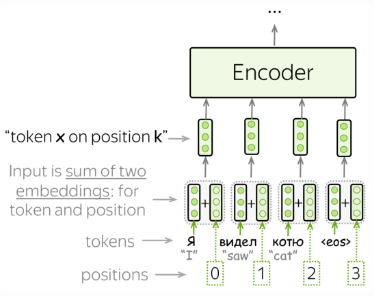
\includegraphics[scale=1]{img/transformer/pos_encoding.png}
    \caption{Positional encoding}
\end{figure}


\subsection{Residual connection}

Как и в сверточных сетях, в Трансформере применяется residual connections. Смысл residual connection очень прост, добавляет входные данные к выходным данным модели, но в то же время это очень полезная вещь: он борется с проблемой затухания градиента по сети и позволяют использовать много слоев.

\begin{figure}[h]
    \centering
    \includegraphics[scale=0.9]{img/transformer/res_block.png}
    \caption{Residual connection}
\end{figure}

В трансформаторе остаточные соединения используются после каждого блока внимания и полносвязного блока.

\newpage

\section{Модель RoBERTa}




\newpage
\chapter{Experiments}

Основной задачей в работе будет классификация видео на наличие юмора с использованием разных моделей для разных модальностей.
Для работы с разными модальностями будут использованы 3 модели, которые были описаны в теоретической части:
\begin{itemize}
    \item Wave2Vec - извлечение аудио признаков,
    \item BERT - извлечение текстовых признаков,
    \item TimeSFormer - извлечение признаков из видео фрагментов,
\end{itemize}

Сначала модели попробуют предсказать классы в своих модальностях, после чего их предсказания будут обработаны вместе для улучшения результатов.

\section{Классификация по одной модальности}

Для извлечения признаков, как уже было описано, будут использоваться 3 различные модели. В силу ограниченных вычислительных мощностей, будут взяты предобученные модели с \href{https://huggingface.co/}{Hugging Face} и дообучены на наших данных.

Так как у нас ровное кол-во наблюдений положительного и отрицательного классов, делим выборку 70\% на дообучение и 30\% валидацию с одинаковым кол-вом примеров разных классов в обеих подвыборках.

Для каждой модели начала посчитаем качество модели по 3 метрикам: Accuracy (из-за отличной балансировки, можем использовать обычную accuracy), Precision, Recall.

\begin{itemize}
    \item Для работы с текстом будем использовать RoBERTa из библиотеки моделей HuggingFace: \href{https://huggingface.co/roberta-base}{roberta-base}.
    \item Для работы с аудио будем использовать Wave2vec2 из библиотеки моделей HuggingFace: \href{https://huggingface.co/facebook/wav2vec2-base}{wav2vec2-base}.
    \item Для работы с видео будем использовать Wave2vec2 из библиотеки моделей HuggingFace: \href{https://huggingface.co/facebook/timesformer-base-finetuned-k400}{timesformer-base}.
\end{itemize}

С помощью предлагаемых Hugging Face интрументов, сделаем дообучение моделей под нашу задачу. \\

\subsection{Результаты}

\textbf{Далее в таблицах с результатами модальности будут называться в сокращенном виде: Текст - Т, Аудио - А, Видео - В.} \\

Результаты классификации по одной модальности: \\

\begin{center}
    \begin{tabular}{ |c||c|c|c|}
        \hline
        \multicolumn{4}{|c|}{Классификация по тексту} \\
        \hline
        Модальность & Accuracy & Precision & Recall   \\
        \hline
        Т           & 0.71377  & 0.70563   & 0.75064  \\
        В           & 0.47836  & 0.50600   & 0.59729  \\
        А           & 0.50885  & 0.57865   & 0.78420  \\
        \hline
    \end{tabular} \\
\end{center}



TimeSFormer показывает достаточно низкие значени метрик, относительно других моделей. Такие результаты связаны со спецификой задачи, моедль не фоксируется только на человеке, но на всем видеофрагменте. Возможным решением станет использование других моделей или инструментов, которые будут обрабатывать именно человека на видео.

Wave2vec показывает хороший recall (т.е модель хорошо угадывает, класс с юмором), но accuracy все еще плохой.

По результатам можем сделать вывод, что самым подходящей для детекции юмора оказалась текстовая модальност, с которой работала RoBERTa. Действительно по тексту легче всего понять, есть ли шутка, потому что не надо обрабатывать много второстепенной информации, как в видео, и "поведение"\ голоса разных людей во время шутки, как на аудио.

\section{Классификация видео с использованием нескольких модальностей}

Теперь попробуем собирать вместе голосование моделей в разных модальностях, сначала будем брать все комбинации 2 модальностей, а потом возьмем 3 модальности.

Подсчет результатов будем производить двумя разными сопобами:
\begin{itemize}
    \item Посчитать среднюю вероятность
    \item Выбирать голосованием, каждой модели за класс
\end{itemize} \\

\subsection{Результаты}

Результаты экспериментов с подсчетом средней вероятности: \\

\begin{center}
    \begin{tabular}{ |c||c|c|c| }
        \hline
        Модальности & Accuracy & Precision & Recall  \\
        \hline
        А + В       & 0.49737  & 0.50512   & 0.60373 \\
        А + Т       & 0.71377  & 0.70488   & 0.75257 \\
        В + Т       & 0.63573  & 0.63569   & 0.66559 \\
        А + В + Т   & 0.63081  & 0.62862   & 0.67074 \\
        \hline
    \end{tabular}
\end{center} \\

В голосованиях в парах и тройке результаты лучше, чем у А и В по одиночке.
А + Т слегка улучшает результат RoBERTa в одиночку, а в остальных парах и тройке, результаты улучшаются, но не достигают RoBERTa.


При спорных ситуациях в голосованием по классам, решающий голос за модальностями с лучшим результатом в прошлой частью (т.е. TimeSFormer имеет самый слабый голос, затем Wave2Vec и самый сильный голос у RoBERTa).

Результаты экспериментов с голосованием по классам: \\

\begin{center}
    \begin{tabular}{ |c||c|c|c|}
        \hline
        Модальности & Accuracy & Precision & Recall  \\
        \hline
        А + В       & 0.49737  & 0.50512   & 0.60373 \\
        А + Т       & 0.71377  & 0.70563   & 0.75064 \\
        В + Т       & 0.71377  & 0.70563   & 0.75064 \\
        А + В + Т   & 0.50885  & 0.50885   & 1.0     \\
        \hline
    \end{tabular}
\end{center} \\

Здесь можно заметить, т.к. текст имеет решщающий голос, то в парах с текстом результаты одинаковые.
В А + В + Т интересно заметить, что recall равен 1.0. Тоесть наша "тройка"\ относит все сэйплы к одному классу.


\chapter{Заключение}

В ходе проделанной работы были прочитаны статьи в разделе нейронных сетей, изучен механизм внимания и архитектура Трансформер с теоретической точки зрения. Также изучены модели, в основе которых лежит Трансформер: RoBerta, используемая для работы с текстовой модальностью, Wave2vec2, используемая для работы с звуковой модальностью, и TimeSFromer, используемая для работы с визуальной модальностью.

Далее были проведены эксперименты  на датасете UrFunnny с каждой из моделей. Изучив результаты можно увидеть, что RoBERTa показыает самые хорошие результаты. Предположения, почему получились такие результаты было сделано в пунке 3.1.1 под таблицей с результатами.

Что касается совмещения результатов моделей (голосование по вероятностям и финальным лэйблам), аудио и текст вместе улучшают результат RoBERTa в одиночку.

Для работы с моделями, обучение и инференс, был изучен фрэймворк HuggingFace, имеющий большую популярность в сфере глубокого обучения. Кроме того были использованы язык программирования Python, PyTorch - бекэнд для нейронных сетей, а также вспомогательные библиотеки librosa (работа со звуком) и Numpy.

Следующим шагом в исследовании детекции юмора может стать объединением моделей в одну, на примере CLIP от openAI или улучшение моделей в аудио и видео модальностях.




\putbibliography %Вместо этой команды будет вставлена библиография

\end{document}